\titre{Questions}
	\begin{itemize}
		\item Java est il entièrement objet ? Non
		\item Une classe est elle un objet en java ? Non
		\item La définition d'une classe est-elle un service dans un LO ? Oui
		\item Un programme est-il un objet dans un LO ? Oui
		\item Les instructions de contrôle existent-elles dans un LO ? Non
	\end{itemize}

\titre{Exemple}\\
	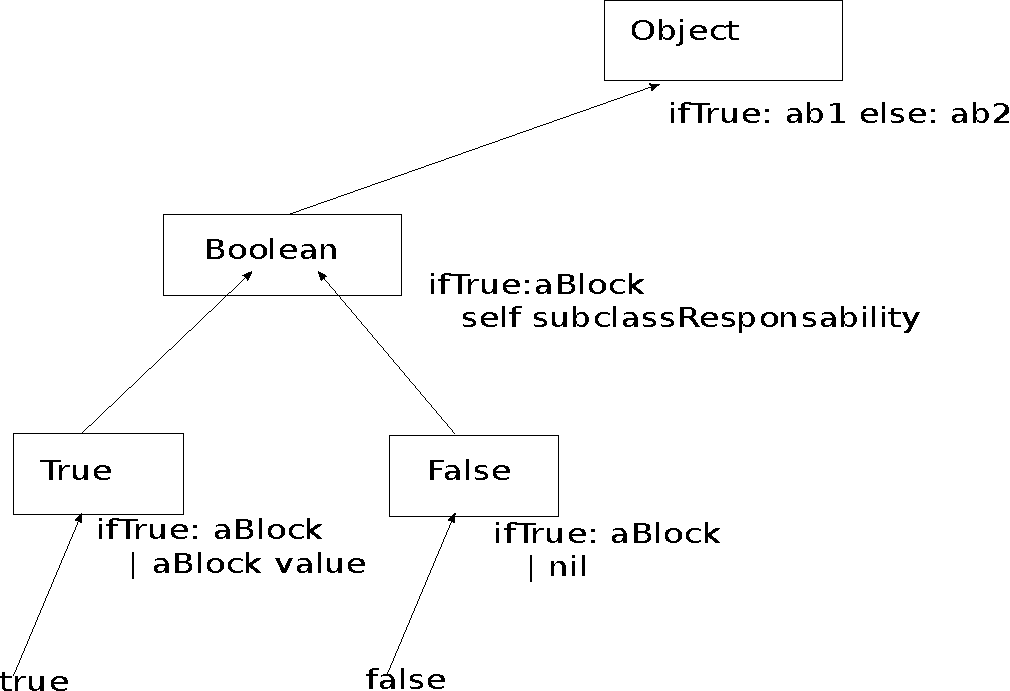
\includegraphics[width=300px]{Images/01_truefalse.pdf}

\titre{Versions possibles :} 2.5, Pharo, Cincom

\titre{Plan du cours :}
	\begin{itemize}
		\item Smalltalk : langage objet
		\item Langage tout objet
		\item Autres caractéristiques (MVC, générateur d'interfaces, objets dépendants, gestion d'erreu, processus)
		\item Travaux pratiques
	\end{itemize}

\titre{Schéma de hiérarchie de smalltalk 76 :}\\
	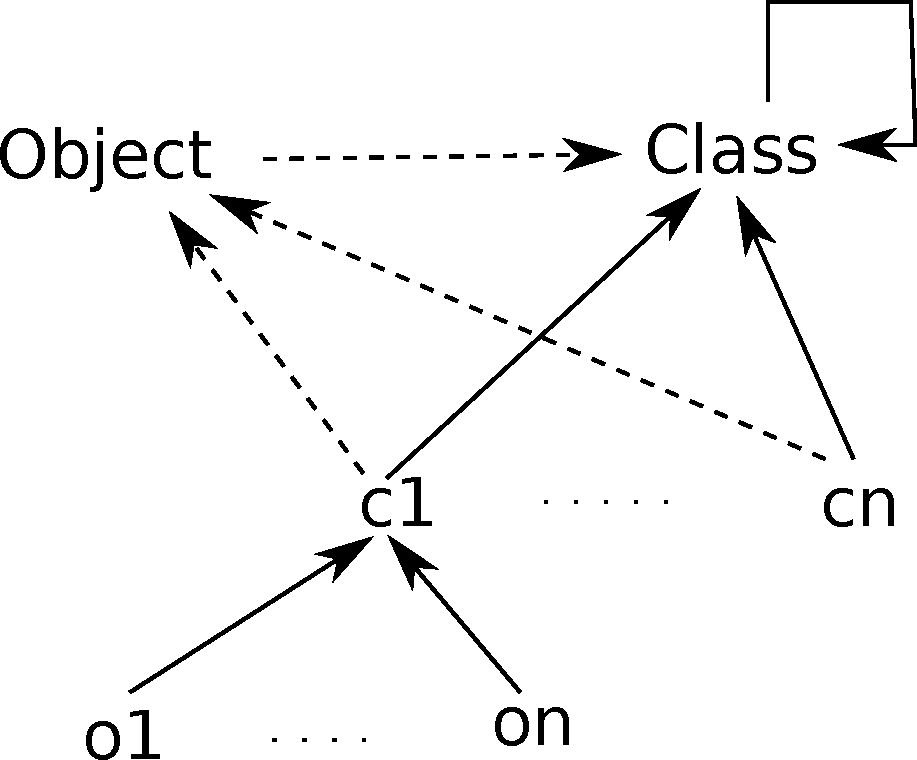
\includegraphics[width=100px]{Images/02_hierarchie.pdf}\\
	Problème : Toutes les classes ont le même comportement (ex : le même constructeur)\\

\titre{Schéma de hiérarchie de smalltalk 80 :}\\ \\
	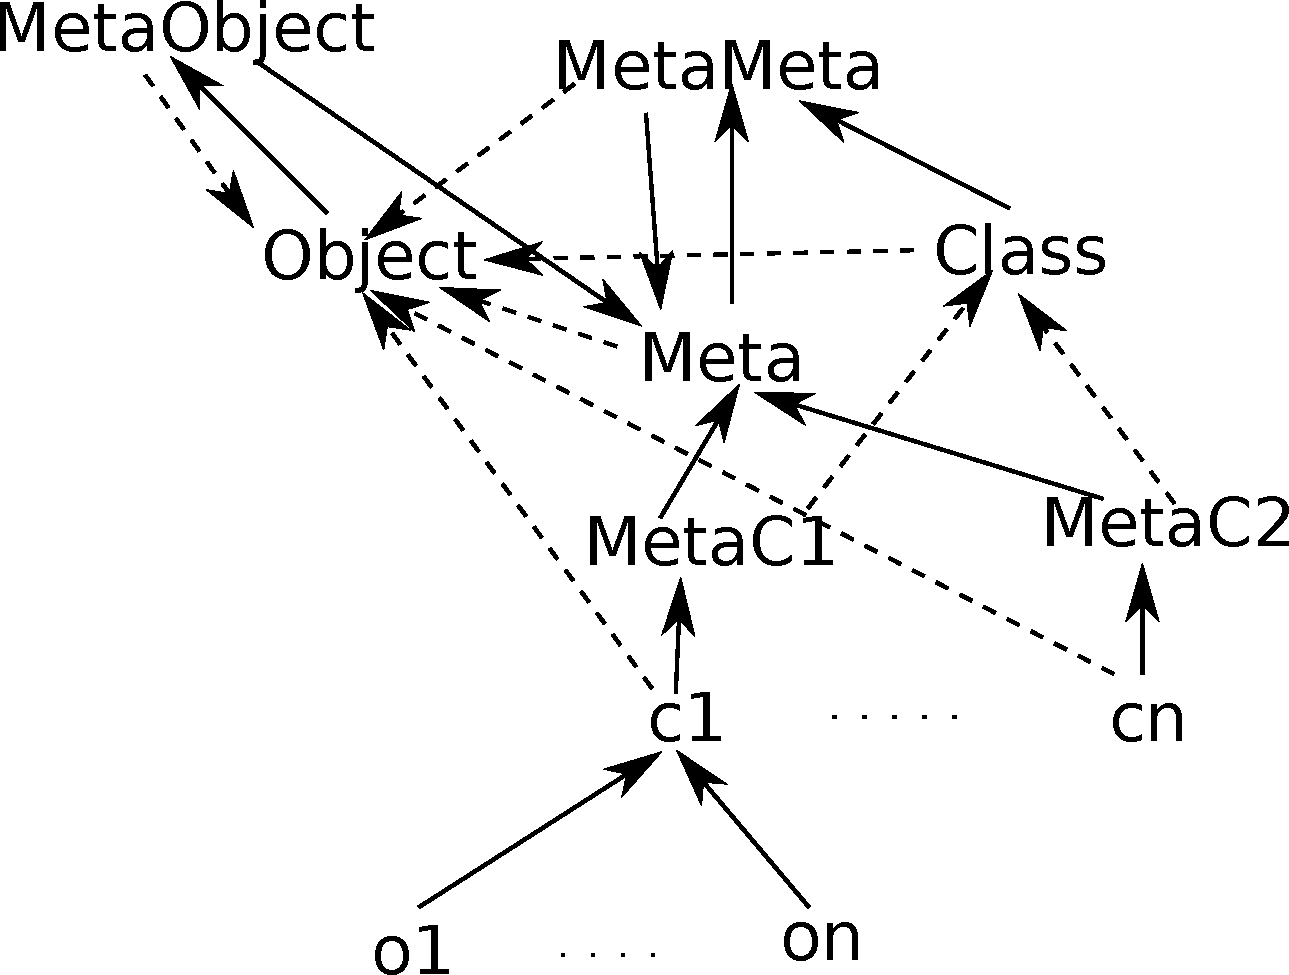
\includegraphics[width=150px]{Images/02_hierarchie2.pdf}\\ \\
	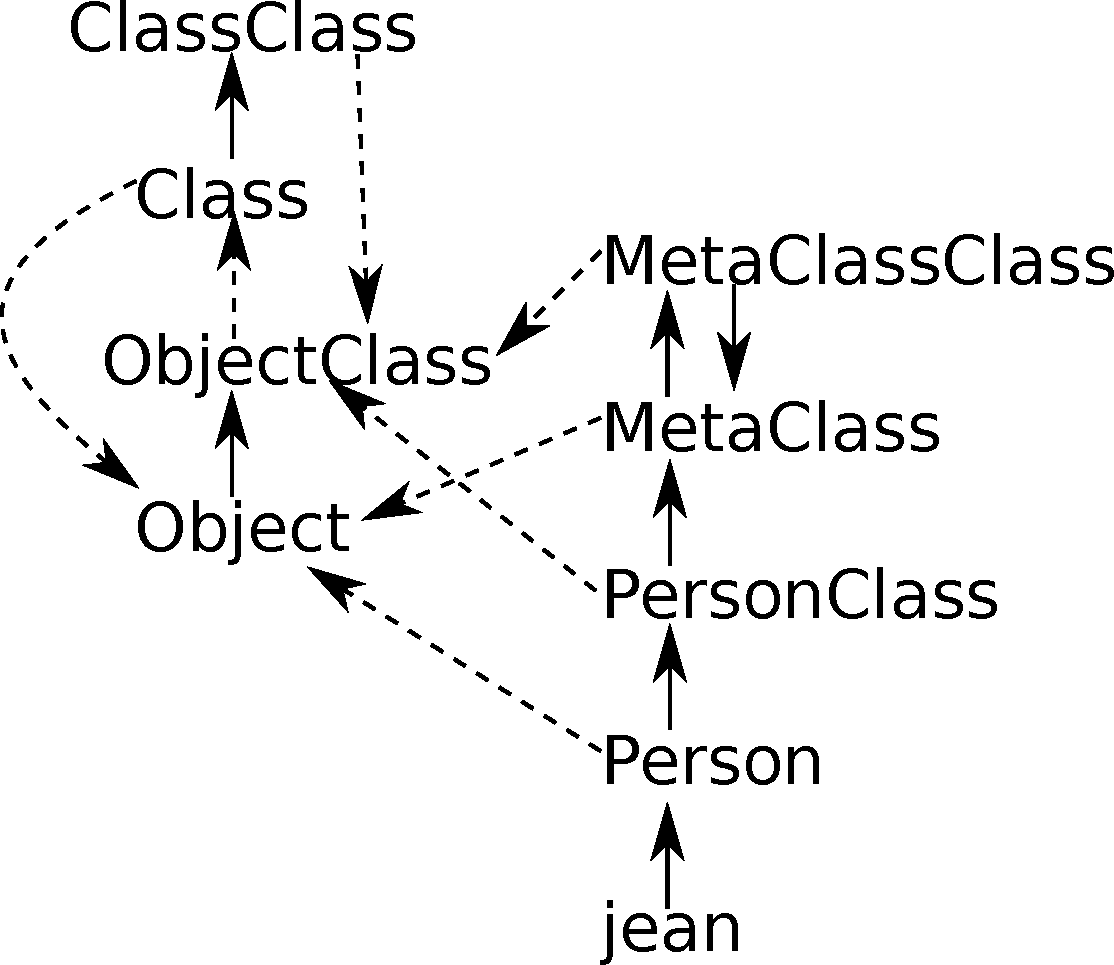
\includegraphics[width=150px]{Images/03_hierarchie3.pdf}\\

\titre{Cas d'utilisation de smalltalk :} Tout domaine nécessitant de l'objet, sans contrainte de temps d'exécution.\\

\titre{Biblio :}
\begin{itemize}
	\item Smalltalk-80 The language and its implementation
	\item Inside Smalltalk
	\item SmallTalk with style
	\item SmallTalk by Example
\end{itemize}
